\documentclass[a4paper,12pt,twoside]{../includes/ThesisStyle}
\usepackage[utf8]{inputenc}
\usepackage[T1]{fontenc}

\usepackage[left=1.5in,right=1.3in,top=1.1in,bottom=1.1in,includefoot,includehead,headheight=13.6pt]{geometry}\renewcommand{\baselinestretch}{1.05}


% =============================================================================
%\usepackage[sectionbib]{chapterbib}	% Cross-reference package (Natural BiB)
%\usepackage{bibunits}
%\usepackage{natbib}					% Put References at the end of each chapter
\usepackage{algorithm}
\usepackage{alltt}
\usepackage{amsfonts}
\usepackage{amsmath}
\usepackage{amssymb}
\usepackage{cite}
\usepackage{color}
\usepackage{enumerate}
\usepackage{booktabs} % used for \midrule
\usepackage{fancyhdr}					% Fancy Header and Footer
\usepackage{graphicx}
\usepackage{ifthen}
\usepackage{latexsym}
\usepackage{multirow}
\usepackage{rotating}					% Sideways of figures & tables
\usepackage{stmaryrd}
\usepackage{subfigure}
\usepackage{url}         
\usepackage{xspace}
\usepackage[normalem]{ulem} % for \sout
\usepackage{xcolor}
\usepackage{tablefootnote}
\usepackage{pifont}

% =============================================================================

% Table of contents for each chapter
\usepackage[nottoc, notlof, notlot]{tocbibind}
\usepackage{minitoc}
\setcounter{minitocdepth}{1}
\mtcindent=15pt

\setcounter{secnumdepth}{3}
\setcounter{tocdepth}{2}
  
% =============================================================================
% Fancy Header Style Options

\pagestyle{fancy}                       % Sets fancy header and footer
\fancyfoot{}                            % Delete current footer settings

%\renewcommand{\chaptermark}[1]{         % Lower Case Chapter marker style
%  \markboth{\chaptername\ \thechapter.\ #1}}{}} %

%\renewcommand{\sectionmark}[1]{         % Lower case Section marker style
%  \markright{\thesection.\ #1}}         %

\fancyhead[LE,RO]{\bfseries\thepage}    % Page number (boldface) in left on even
% pages and right on odd pages
\fancyhead[RE]{\bfseries\nouppercase{\leftmark}}      % Chapter in the right on even pages
\fancyhead[LO]{\bfseries\nouppercase{\rightmark}}     % Section in the left on odd pages

\let\headruleORIG\headrule
\renewcommand{\headrule}{\color{black} \headruleORIG}
\renewcommand{\headrulewidth}{1.0pt}
\usepackage{colortbl}
\arrayrulecolor{black}

\fancypagestyle{plain}{
  \fancyhead{}
  \fancyfoot{}
  \renewcommand{\headrulewidth}{0pt}
}


% =============================================================================
% Clear Header Style on the Last Empty Odd pages
\makeatletter

\def\cleardoublepage{\clearpage\if@twoside \ifodd\c@page\else%
  \hbox{}%
  \thispagestyle{empty}%              % Empty header styles
  \newpage%
  \if@twocolumn\hbox{}\newpage\fi\fi\fi}

\makeatother

\newenvironment{maxime}[1]
{
\vspace*{0cm}
\hfill
\begin{minipage}{0.5\textwidth}%
%\rule[0.5ex]{\textwidth}{0.1mm}\\%
\hrulefill $\:$ {\bf #1}\\
%\vspace*{-0.25cm}
\it 
}%
{%

\hrulefill
\vspace*{0.5cm}%
\end{minipage}
}

\let\minitocORIG\minitoc
\renewcommand{\minitoc}{\minitocORIG \vspace{1.5em}}


\renewcommand{\epsilon}{\varepsilon}

% centered page environment
\newenvironment{vcenterpage}
	{\newpage\vspace*{\fill}\thispagestyle{empty}\renewcommand{\headrulewidth}{0pt}}
	{\vspace*{\fill}}
	

%=============================================================================

\usepackage{needspace}
\newcommand{\needlines}[1]{\Needspace{#1\baselineskip}}

\usepackage{xcolor}
\definecolor{source}{gray}{0.95}
% source code formatting
\usepackage{listings}
    % global settings for source code listing package
\lstset{
    basicstyle=\ttfamily\small,
    showspaces=false,
    showstringspaces=false,
    captionpos=b, 
    columns=fullflexible}

\lstdefinelanguage{ST}{
    keywordsprefix=\#,
    morekeywords=[0]{true,false,nil},
    morekeywords=[1]{self,super,thisContext},
    morekeywords=[2]{ifTrue:,ifFalse:,whileTrue:,whileFalse:,and:,or:,xor:,not:,by:,timesRepeat:},
    sensitive=true,
    morecomment=[s]{"}{"},
    morestring=[d]',
    escapechar={!},
    alsoletter={., :, -, =, +, <},
    moredelim=**[is][\itshape]{/+}{+/},
    literate=
        {^}{{$\uparrow$}}1
        {:=}{{$\leftarrow$}}1
        {~}{{$\sim$}}1
        {-}{{\sf -\hspace{-0.13em}-}}1  % the goal is to make - the same width as +
        {+}{\raisebox{0.08ex}{+}}1		% and to raise + off the baseline to match V
        , % Don't forget the comma at the end!
    style=STStyle
}
\lstdefinestyle{STStyle}{
    tabsize=4,
    %frame=leftline,
    % frame=bl,
    %framerule=2pt,
    %rulecolor=\color{gray},
    % backgroundcolor=\color{white},
    %backgroundcolor=\usebeamercolor[bg]{listing},
    basicstyle=\ttfamily\small,
    keywordstyle=\bf\ttfamily,
    % stringstyle=\color{orange},
    stringstyle=\mdseries\slshape,
    commentstyle=\it\rmfamily\color{darkgray}, 
    commentstyle=\mdseries\slshape\color{gray},
    %commentstyle=\mdseries\slshape,
    emphstyle=\bf\ttfamily,
    escapeinside={!}{!},
	%backgroundcolor=\color{source},
    %emphstyle={[2]\color{red}},
    %emphstyle={[3]\color{blue}\bf},
    %emphstyle={[4]\color{blue}},
    keepspaces=true
} 

%\lstnewenvironment{javacode}  [1][]{\lstset{language=java,#1}\needlines{#2}}{} 
%\lstnewenvironment{pythoncode}[2][]{\lstset{language=python,#1}\needlines{#2}}{}
\lstnewenvironment{stcode}    [2][]{\lstset{language=ST,#1}\needlines{#2}}{}
\lstnewenvironment{ccode}     [2][]
    {\lstset{language=C,numbers=left,escapechar=\$,numberstyle=\tiny,#1}\needlines{#2}}{}

% ON: I tried to pass the line number options in as arg #1 but it does not work for me
% I also could net get the line numbers to consistently increase
\lstnewenvironment{numstcode} [2][]
    {\lstset{language=ST,numbers=left,numberstyle=\tiny,numbersep=2pt,#1}\needlines{#2}}{}
\lstnewenvironment{numstcodecont} [2][]
    {\lstset{language=ST,numbers=left,numberstyle=\tiny,numbersep=2pt,firstnumber=last#1}\needlines{#2}}{}

\newcommand{\lst}[1]{{\tt #1}}

% In-line code (literal)

% In-line code (latex enabled)
% Use this only in special situations where \ct does not work
% (within Section headings ...):
\newcommand{\lct}[1]{{\textsf{\textup{#1}}}}
% Code environments
\lstnewenvironment{code}{%
	\lstset{%
		% frame=lines,
		frame=single,
		framerule=0pt,
		mathescape=false
	}
}{}

%\renewcommand{\lstlistingname}{Code Example}

% =============================================================================
\newboolean{showcomments}
\setboolean{showcomments}{true}

\ifthenelse{\boolean{showcomments}} {
	\newcommand{\ugh}[1] {\textcolor{red}{\uwave{#1}}}	% please rephrase
	\newcommand{\ins}[1] {\textcolor{blue}{\uline{#1}}}	% please insert
	\newcommand{\del}[1] {\textcolor{red}{\sout{#1}}}	% please delete
	\newcommand{\chg}[2] {								% please change
		\textcolor{red}{\sout{#1}}{\ra}
		\textcolor{blue}{\uline{#2}}}
	\newcommand{\nbc}[3]{								% comment
		{\colorbox{#3}{\bfseries\sffamily\scriptsize\textcolor{white}{#1}}}
		{\textcolor{#3}{\sf\small$\blacktriangleright$\textit{#2}$\blacktriangleleft$}}}

}{
	\newcommand{\ugh}[1]{#1}							% please rephrase
	\newcommand{\ins}[1]{#1}							% please insert
	\newcommand{\del}[1]{}								% please delete
	\newcommand{\chg}[2]{#2}							% please change
	\newcommand{\nbc}[3]{}								% comment
}

% =============================================================================
\usepackage[pagebackref,hyperindex=true]{hyperref}


% Links in pdf
\usepackage{color}
\definecolor{linkcol}{rgb}{0.0, 0.0, 0.0} 
\definecolor{citecol}{rgb}{0.0, 0.0, 0.0} 

% Change this to change the informations included in the pdf file
% See hyperref documentation for information on those parameters
\hypersetup {
	bookmarksopen=true,
	pdftitle="Design and Use of Anatomical Atlases for Radiotherapy",
	pdfauthor="Olivier COMMOWICK", 
	pdfsubject="Creation of atlases and atlas based segmentation", %subject of the document
	%pdftoolbar=false, % toolbar hidden
	pdfmenubar=true, %menubar shown
	pdfhighlight=/O, %effect of clicking on a link
	colorlinks=true,
	pdfpagemode=UseNone,
	pdfpagelayout=SinglePage,
	pdffitwindow=true,
	linkcolor=linkcol,
	citecolor=citecol,
	urlcolor=linkcol
}

% =============================================================================
\newcommand{\figlabel}[1] {\label{fig:#1}}
\newcommand{\chaplabel}[1]{\label{chap:#1}}
\newcommand{\seclabel}[1] {\label{sec:#1}}
\newcommand{\tablabel}[1] {\label{tab:#1}}
\newcommand{\lstlabel}[1] {\label{lst:#1}}

\newcommand{\figref}[1] {Figure~\ref{fig:#1}}
\newcommand{\chapref}[1]{Chapter~\ref{sec:#1}}
\newcommand{\secref}[1] {Section~\ref{sec:#1}}
\newcommand{\tabref}[1] {Table~\ref{tab:#1}}
\newcommand{\lstref}[1] {Listing~\ref{tab:#1}}

\newcommand{\commented}[1]{}

\newcommand{\bs}    {\symbol{'134}} % backslash
\newcommand{\us}    {\symbol{'137}} % underscore
\newcommand{\ttt}[1]{\texttt{#1}}
\newcommand{\ie}    {\emph{i.e.},\xspace}
\newcommand{\eg}    {\emph{e.g.},\xspace}
\newcommand{\etal}  {\emph{et al.}\xspace}
\newcommand{\ns}    {\!\!\!\!} %big negative space
\newcommand{\cnull} {\textbackslash0\xspace}


\newcommand\fix[1]{\nb{FIX}{#1}}
\newcommand\todo[1]{\nb{TO DO}{#1}}
\newcommand\cb[1]{\nbc{CB}{#1}{purple}}
\newcommand\sd[1]{\nbc{SD}{#1}{orange}}
\newcommand\is[1]{\nbc{IS}{#1}{gray}}
\newcommand\gc[1]{\nbc{GC}{#1}{olive}}
\newcommand\ct[1]{\nbc{CT}{#1}{teal}}
\newcommand\md[1]{\nbc{MD}{#1}{blue}}
\newcommand\dc[1]{\nbc{DC}{#1}{green}}

% =============================================================================
\newcommand{\NBFFI}  {Native\-Boost-FFI\xspace}
\newcommand{\NB}  {Native\-Boost\xspace}
\newcommand{\B}   {Benzo\xspace}
\newcommand{\ST}  {Small\-talk\xspace}
\newcommand{\PH}  {Pharo\xspace}
\graphicspath{{.}{../figures/}}

\begin{document}
% =============================================================================

\chapter{Benzo}
\chaplabel{benzo}
\minitoc

% =============================================================================

% ===========================================================================
\section{Introduction}
\seclabel{introduction}
% ===========================================================================
High-level low-level programming \cite{Fram09a} encourages to use high-level languages such as Java to build low-level execution infrastructures or to do system programming. 
It is successfully used in experimental high-level self-hosted virtual machines (VMs) such as Jikes~\cite{Alpe99a}.  
Frampton et al. present a framework that is biased towards a statically typed high-level language, taking strict security aspects into account.
Their approach promotes to address low-level system programming tasks with the tools and abstractions of high-level languages.
However, their solution has reduced applicability in a dynamic and reflective context.
By reflective, we refer to the combined capabilities to inspect (introspection) and change (intercession) the same execution concepts at runtime \cite{Maes87a}.

From a reflective point of view it seems natural to dynamically modify the VM at runtime and not just at compile-time.
If we are able to modify the VM from language-side we blur the line between these two distinct worlds, becoming indistinguishable to talk about the VM or the language-side.
Hence throughout this paper we use the term language runtime to refer to the running VM combined with the language-side application.


%Extending high-level language VM is difficult due to their static low-level construction which usually shares little resemblance with the language-side.
%Yet for tasks, like the previously presented primitive instrumentation, if we want to tackle it with a high-level language, we need solid low-level interaction.
%\cb{some more context missing here}

\subsubsection{Requirements.}
Extending the VM is only one particular case of modifying or extending the complete language runtime.
Language-side libraries, reflective capabilities, VM extensions or hybrid approaches are other possibilities which we discuss in detail in Section~\secref{related}.
All these typical extension mechanisms are not sufficient if we want to modify the VM from language-side, or in our terminology, to reflectively modify the language runtime. Furthermore these mechanisms are based on the fact that there is a clear barrier between language and VM.
A solution that crosses these barriers requires the following properties:

%interface to interact with low-level code.
%To stay flexible and compatible enough a generic solution should add these new key features with as little static low-level intrusion as possible.

\begin{enumerate}
	\item It must be \emph{reflective} in the sense it must support \emph{dynamic} changes of the language runtime (VM) without requiring a system restart.
	\item It should imply minimal changes to the existing low-level runtime to \emph{considerably reduce development efforts}.
\end{enumerate}


\subsubsection{\B a Framework for Reflective Low-level Programming.}

High-level low-level programming is a powerful technique for system programming without resorting to static low-level environments \cite{Fram09a,Wimm13a} that \ugh{almost} fulfills our requirements.
However, in a reflective setup it fails to comply with the first requirement mentioned in the previous paragraph: it does not allow reflective changes at runtime.
Our approach for overcoming this limtation consists of \B, a lightweight and reflective framework that dynamically generates native code from language-side and allows its execution on the fly.
It relies only on a small set of generic VM extensions described in Section~\secref{vm-requirements}, whereas the vast majority of the framework is implemented as a language-side library.

\subsubsection{\B Applications.}
In Section \secref{usecase} we advocate the contribution of this approach by providing three different incremental examples that heavily use the framework.
Unlike typical implementations that would focus on writing them as VM extensions, we implement them completely at language-side using \B:
%\ugh{They rely on it} for extending or even improving language runtime capabilities.

%\begin{description}[noitemsep]
\begin{description}
	\item[FFI] A complete language-side Foreign Function Interface (FFI) implementation, described in Section \secref{ffi}.
	\item[Dynamic Primitives] A language-side compilation toolchain that replaces system primitives at runtime with customized code, described in Section \secref{waterfall}. 
	\item[Language-side JIT Compiler] A JIT compiler that works at language-side and interacts with the VM for code synchronization, described in Section \secref{nabujito}
\end{description}


\noindent Illustrated by these three distinct examples, the contributions of this paper are:
\begin{enumerate} 
	\item A \emph{reflective} high-level low-level programming framework that encourages the extension of high-level language runtimes on the fly without the overheads imposed by pure high-level solutions. 
	%\item The framework promotes open interactions with the low-level world .
	\item A proof of concept of the proposal with the implementation and description of three different tools that heavily use reflective low-level programming and covers distinct scenarios.
\end{enumerate}


%\subsection{Use Case: Dynamic Primitive Instrumentation}
%\md{Remove use-case here and inline in 1.2 Bridging abstraction layers}
%\noindent To illustrate this limitation we take the example of dynamically intercepting VM primitives. In most managed language runtimes, VM primitives are used for essential tasks such as object creation or provide fundamental functionality that can not be obtained otherwise at language-side~\cite[page 52]{Gold83a}. Already the simple example of measuring the time spent in an essential primitive while executing a performance critical task is difficult to do efficiently.


%Reflective solutions at language-side could take advantage of the intercession capabilities that allow changing or augmenting almost any behavior at runtime. In practice, this does not work for primitives. In addition, reflectively measuring the duration of the time primitive itself will easily cause meta-recursion. Hence in general reflective instrumentation will not work on primitives used for the instrumentation itself. Thus efficiently instrumenting VM primitives in a dynamic and reflective environment is not feasible in many cases.

%Naturally, if we leave the high-level realm there are efficient tools at hand for instrumentation. Existing solutions for efficient low-level instrumentation such as DTrace~\cite{Coop12a} work by installing static hooks. Though in a reflective language assumptions can change at runtime and thus static solutions are not appropriate. At the same time we clearly see that such instrumentation is not a typical high-level application. To combine these two worlds we need a different approach.


% ===========================================================================
\section{The \B Framework}
\seclabel{benzo}
% ===========================================================================
\B is implemented in \PH\footnote{\url{http://pharo.org}}, a \ST inspired language.
\PH comes with all the reflective capabilities known from \ST where most language-side components can be altered dynamically.
\B is implemented at language-side and only requires the help of two simple and generic primitives to activate \cb{ad-hoc has a negative conotation} native code and resolve the entry point address position of referenced C functions.

%----------------------------------------------------------------------------
\subsection{VM Context}
\seclabel{vm-requirements}
%----------------------------------------------------------------------------
\PH emerged from the Squeak project \cite{Inga97a}.
The \PH VM (Cog) implementation \cite{Mira11a} also evolved from the original Squeak bytecode interpreter.
The current VM uses a moving Garbage Collector (GC) with two generations\gc{ref?} and uses a JIT that applies basic register allocation to reduce stack load. 
This situation is not a direct requirement for \B but it is assumed as given and thus not further discussed in detail.
However, \B requires certain features that were not supported in the existing VM implementation.
Mainly our requirement is being able to generate executable code and activate it at runtime.
This is general and essential so it applies to any VM that wants to support dynamic code execution managed at language-side.

%----------------------------------------------------------------------------
\subsubsection{Executable Memory.}
\seclabel{exeutable-memory}
 
We use standard \ST objects to hold the generated native code.
However, by default the object memory is not executable.
This leaves two choices: mark the whole object memory executable or only move the objects with the native code to a special executable memory region.
We took the path of least resistance and marked the whole object memory as executable.
The other solution requires substantial changes for memory management. As the VM has a moving GC we only access high-level \ST objects via an indirection from low-level code.
Another approach would have been to harness the fixed sized executable region used by the existing JIT.
However, the JIT space does not hold normal \ST objects but special low-level structures and uses its own special GC. 

%----------------------------------------------------------------------------
\subsubsection{VM Interaction.}
\seclabel{vm-interaction}

The standard way in \ST to execute low-level code is to use a tag in the method definition. The following example shows such a method on the \ttt{Float} class.
%
\begin{stcode}[label={lst:basic-primitive}]{5}
* aNumber 
	<primitive: 49>
	^ aNumber adaptToFloat: self andSend: #*
\end{stcode}
%
Here we use the primitive 49 to call a VM function which efficiently multiplies two floats. 
%Figure~\figref{smalltalkPrimitive}-a describes the case where the primitive is successfully executed.
However, if the primitive is unable to do the operation, for instance if the argument \ttt{aNumber} is not a float, it will signal a failure which causes the VM to execute the fallback \ST code in the method body.  
%Fig.~\figref{smalltalkPrimitive}-b describes it. 

%\begin{figure}[ht]
%	\centering
%	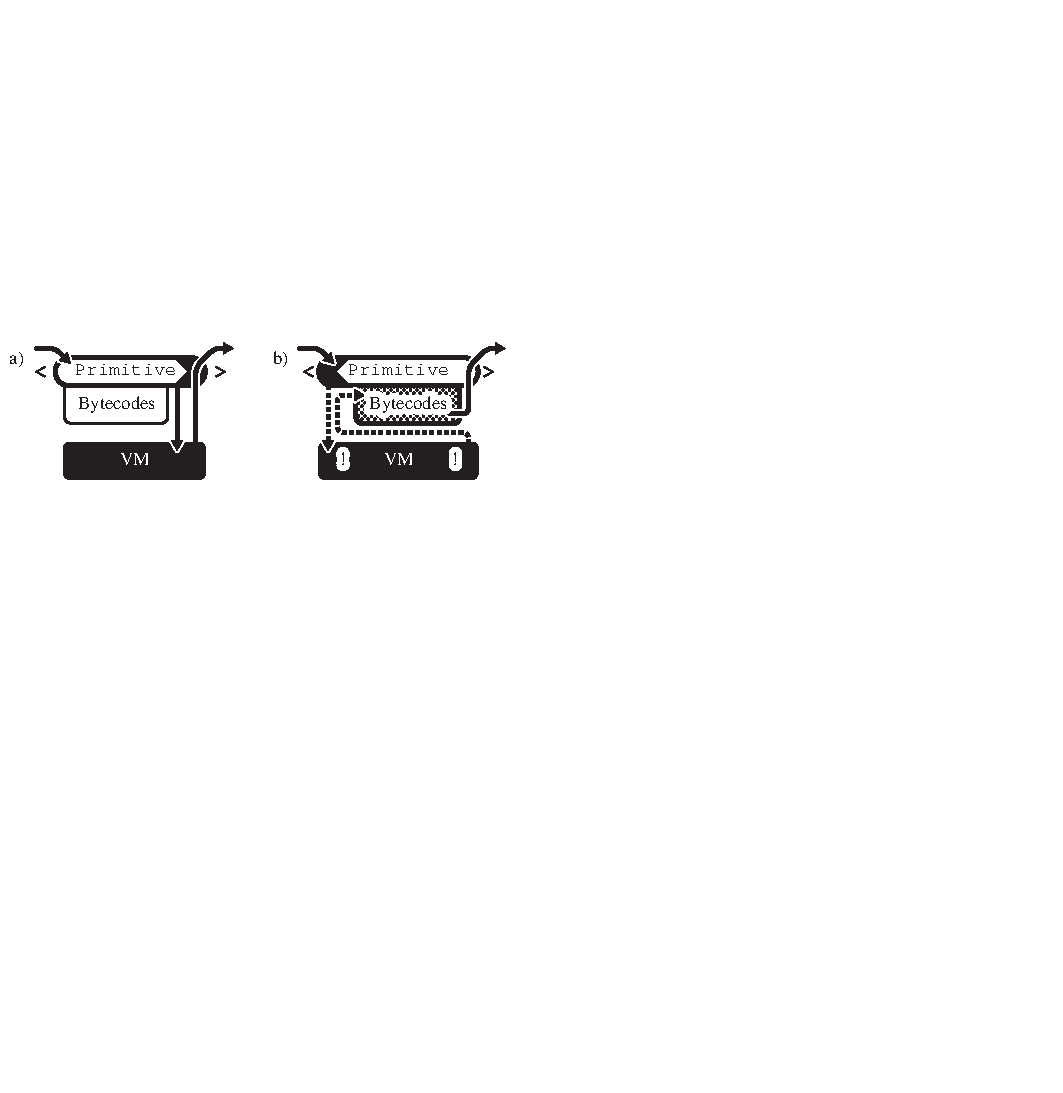
\includegraphics{smalltalkPrimitive}
%	%\nocaptionrule
%	\caption{Generic primitive methods in \PH: a) A primitive completely bypasses the bytecode, b) A failing primitive executes the \ST bytecode as fallback.}
%	\figlabel{smalltalkPrimitive}
%\end{figure}


\B uses the primitives as a gate to enter the low-level world from the language-side.
Our custom primitive then executes the generated native code and returns to language-side. 
This code is appended inside the compiled method object.
When the primitive is activated, it  accesses the currently executed compiled method via a VM function. Figure \figref{nativeCodeMethod} shows the structure of a \ST compiled method that has native code attached to it.
We see the primitive tag on top, followed by the literal frame which holds references to symbols and classes used in the method.
The subsequent \ST bytecode is the fallback code executed only if the primitive fails. Only then appears the native instructions.
A marker at the end of the compiled method called trailer type is used to flag methods that actually have native code attached to them.
%
\vspace{-1mm}
\begin{figure}[ht]
	\centering
	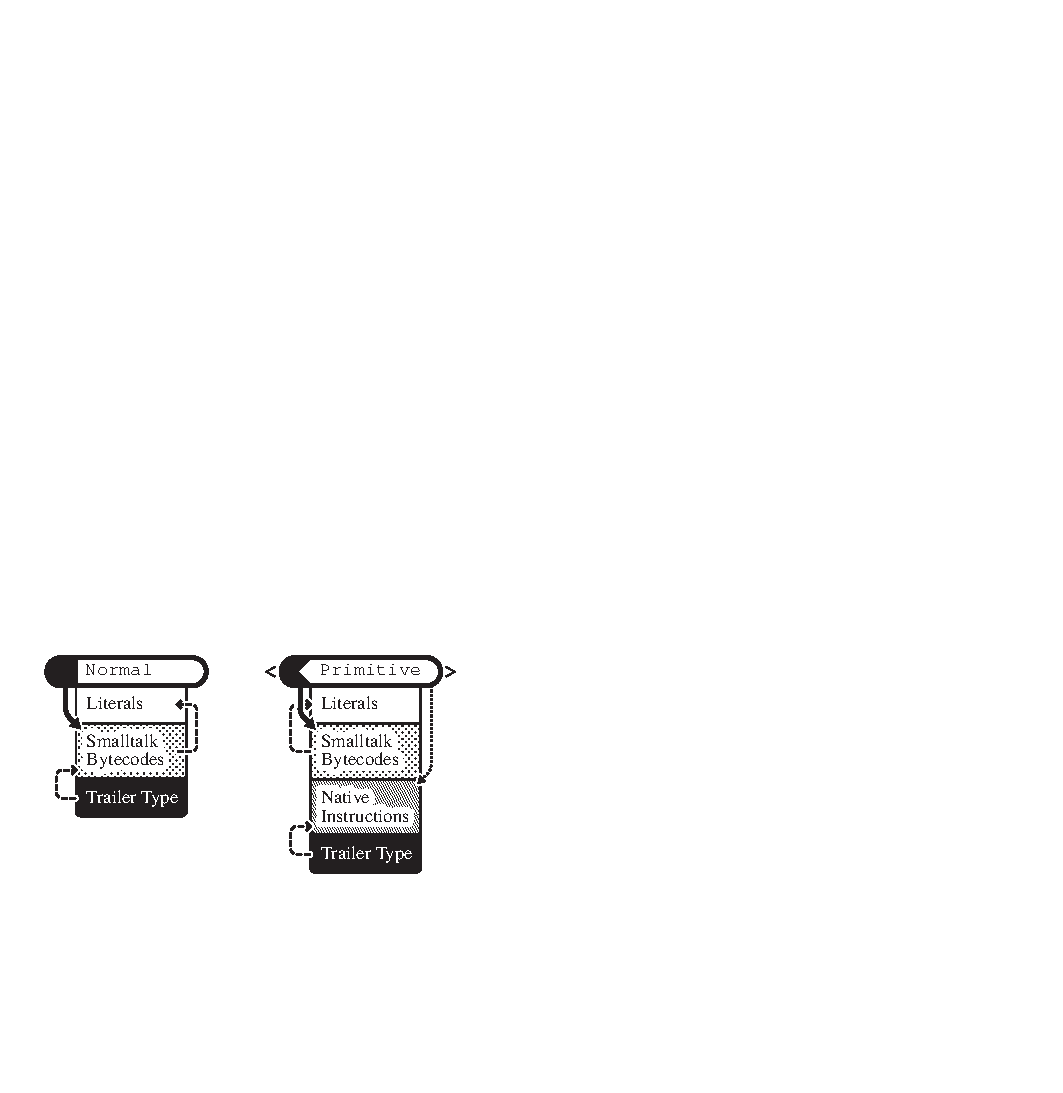
\includegraphics[scale=0.8]{nativeCodeMethod}
	%\nocaptionrule
	\caption{A standard \ST compiled method on the left and a method with appended native instructions generated by \B.}
	\figlabel{nativeCodeMethod}
\end{figure}
\vspace{-3mm}

Since compiled methods are first-class objects it is possible to modify them at runtime and append the native code.
The primitive \ttt{primitiveNativeCall}, which is implemented by \B, is the responsible of running the native instructions in a \ST method.
The code example \ttt{interrupt3} shows a very basic application of our infrastructure.
In Section \secref{benzo-language-side}, through more detailed examples, we describe how \B uses \ST code to generate the native instructions.
%
\begin{stcode}[label={lst:basic-native-code}, caption={\ST method using \B for very basic low-level debugging.}, escapeinside={@}{@}]{5}
interrupt3
	<primitive: 'primitiveNativeCall' 
	 module: 'BenzoPlugin' >
	Benzo generate: [ :asm | asm int3 ]
\end{stcode}
\vspace{-5mm}

%----------------------------------------------------------------------------
\subsubsection{Native Code Platform Interaction.}
\seclabel{platform-interaction}

To ensure that the code is compatible with the current platform a VM specific marker is expected at the beginning of the native code on the compiled method.
Upon activation \B compares this marker with the one from the current VM.
If they don't match, \B signals a failure that causes the VM to evaluate the fallback \ST code.
With this elegant approach \B regenerates native code lazily on new platforms.
Moreover, it does not have to flush the native code when the application is restarted on the same platform.

%----------------------------------------------------------------------------
\subsubsection{Garbage Collector Interaction.}
\seclabel{gc-interaction}
%Compiled methods in \PH have a special section, the literal frame, which stores objects referenced in the bytecodes.
%Bytecodes then only have indirect access to these objects by indexing into the literal frame.
%This simplifies the implementation of the garbage collector as it only has to scan the beginning of each method for possible references to objects. 
%So the GC only tracks \ST objects when they are in the method literal frame. 
The moving GC of the VM used for \PH has a significant impact on the low-level code we can generate using \B.
For instance it is not possible to statically refer to language-side objects from native code as object addresses change after each garbage collection.
Modifying the GC to support regions of non-moving objects would solve this problem.
However, we chose to minimize the number of low-level VM modification necessary to run our experiments and opted for a simpler solution.
\B accesses language-side objects through an indirection.
For indirectly accessing objects the Pharo VM already features a special structure, named \emph{external roots}.
This array has a fixed-location in memory which can be used to access moving language-side objects.
The GC updates the addresses in this VM structure after each run.
Hence we have the static address of the external roots object as an entry point to statically access \ST objects.
%
\vspace{-2mm}
\begin{figure}[ht]
	\centering
	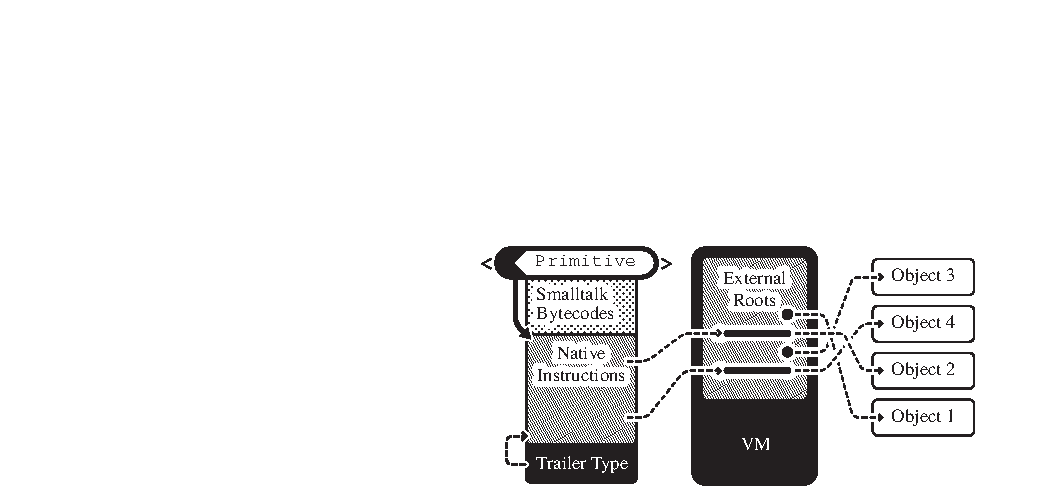
\includegraphics[scale=0.8]{externalRoots}
	%\nocaptionrule
	\caption{Pointers to objects registered as external roots are pinpointed at fixed offset in global VM-level object.
	}
	\figlabel{externalRoots}
\end{figure}
\vspace{-3mm}
%
Summarizing, for accessing \ST objects within native code we first register it as an external root object and access it only indirectly.
This means that for native code, instead of a method-local literal array we share a global literal array as shown in Figure \figref{externalRoots}. 
\B only adds an \ttt{Array} to the external root objects which is managed from language-side and administers all references.

%\revc{The external roots concept appears here first but the idea of "indirection" has been mentioned. The regular literal frame of compiled methods are discussed heavily; that would suggest that the generated native code could use relative offset from the code location and still be able to "pin-point" the literal slot in the literal frame. What is the downside of this approach? (And how slots in the external roots garbage collected?)}
%\gc{I'm not very interested with the comment above. But perhaps here it is a good place to say that once the native code start executing our VM assures that a GC could not happen}
%----------------------------------------------------------------------------
\subsubsection{JIT Interaction.}
\seclabel{jit-interaction}

When the Pharo VM starts the execution of dynamic generated code the execution environment changes slightly.
Similarly, when entering primitives or plugin code, the managed execution mode is left and a normal C-level execution environment is reestablished until the primitive finishes and the VM jumps back to the jitted code. 
To avoid these context changes that imply a considerable performance overhead, we extend the VM to support inlining of native code in the JIT phase following the same strategy as other existing primitives which are inlined at JIT-level.
The \B prologue and epilogue used for managing the low-level stack are replaced by an adapted version for the JIT.
The performance boost of this optimization is further discussed in Section \secref{issues-performance}.

%----------------------------------------------------------------------------
\subsubsection{Error Handling.}
\seclabel{error-handling}

\B provides an error handling facility that allows to return high-level error messages from the low-level code. 
The native code builder provides a helper method called \ttt{failWithMessage:} 
that generates the proper assembler instructions to return a full error message.
This allows plugins to return clear and meaningful error codes, improving the debugging tasks and enabling a better interaction with users.

%\reve{does a call to "failWithMessage:" result in an exception being thrown, or does it just display an error message. The former would be more useful b/c it would enable language-side code to catch the exception and do something about it, but the paper doesn't make it clear that this is the case.}


%----------------------------------------------------------------------------
\subsection{\B's Language-Side Implementation}
\seclabel{benzo-language-side}
%----------------------------------------------------------------------------
As a key design decision, we determine to keep the interface to the low-level world minimal.
The following describes the features of \B at the high-level language-side.

%----------------------------------------------------------------------------
\subsubsection{Code Generation.}
\seclabel{code-generation}

\B delegates native code generation to a full assembler written in \ST. The following example shows how to use the assembler to generate the native code for moving \ttt{1} into the 32-bit register \ttt{EAX}.
%
\begin{stcode}{4}
Benzo x86 generate: [ :asm |
	asm mov: 1 asUImm to: asm EAX ].
\end{stcode}
%
The implementation first creates a slightly more abstract intermediate format.
The abstract operations can be extended by custom operations that may expand to several native instructions. For pragmatic reasons current implementation only supports \textsc{x86} and \textsc{x86-64}.
%
%	\reve{You claim that the "assembler is platform-agnostic", but how so? In the examples, you seem to use instructions that are clearly x86-specific, e.g., MOVs involving EAX. On a related note, you say in the same section that "there are plans to improve the platform independence by implementing a more abstract DSL for NativeBoost."}
%
The full features of the high-level environment are available when generating native code.
Hence complex instruction sequences can easily be delegated to other objects.
In the following example we use a VM helper to instantiate an array. It is worth noting that all are standard message sends:
%
\begin{stcode}{5}
Benzo x86 generate: [ :asm :helper | | register |
	register := helper classArray.
	register := helper 
		instantiateClass: register
		indexableSize: 10
	asm mov: register to: asm resultRegister ].
\end{stcode}
%
The VM helper exposes a basic, low-level interface to access objects and its properties.
Additional methods cover the access to the external roots described in Section \secref{gc-interaction}.
In this case the \ttt{\#instantiateClass:indexableSize:} will generate the proper native code to call to a VM function and make sure that the side-effects of a possible GC run are handled properly.
By default the value in the result register is returned back to the language-side. On \textsc{x86} this defaults to \ttt{EAX}.
In section \secref{usecase} we introduce more substantial applications based on \B.

%----------------------------------------------------------------------------
\subsubsection{Code Activation.}
\seclabel{code-activation}
 
A \B primitive is responsible for the native code activation which consists of three main steps:
%
%\begin{itemize}[noitemsep,nolistsep] 
\begin{enumerate}
	\item Check if there is native code in the actual compiled method and if it is compatible with the current platform.
	\item Generate native code if necessary.
	\item Activate the native code for execution.
\end{enumerate}
%
The example in Listing \lstref{basic-native-code} uses \B's generator to create and install the native code which would trigger a low-level interrupt. Behind the scenes \B adds some more information to the code as the already mentioned platform marker. 
For activation \B uses reflective features to restart the method containing the native code.
Upon the second activation, after already generating the native code, \B moves the native code to the end of the compiled method and activates it.
This mechanism is shown in Figure \figref{nativeCodeActivation}.

\begin{figure}[ht]
	\centering
	%[scale=0.9]
	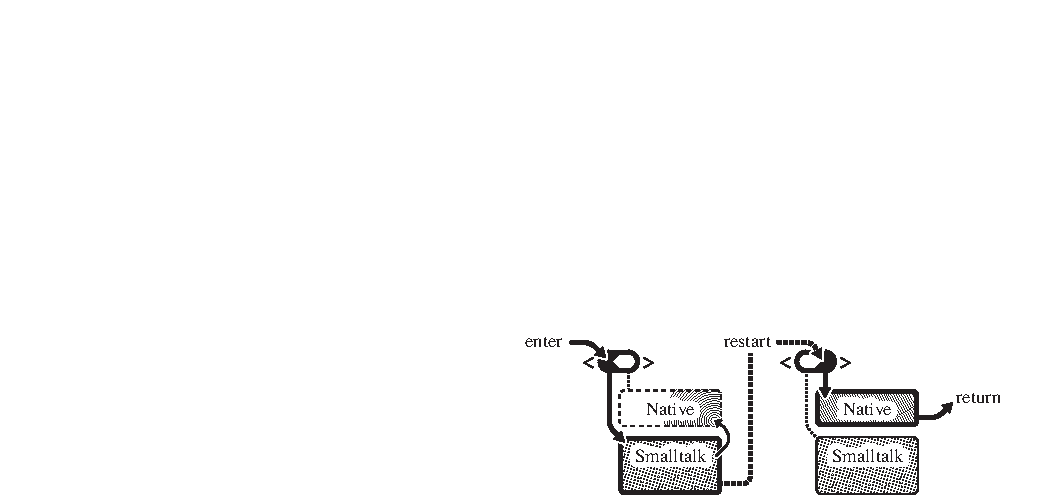
\includegraphics{nativeCodeActivation}
	\caption{Native code activation with \B: The first call triggers the code generation. Then the method is restarted and the native code executed.}
	\figlabel{nativeCodeActivation}
\end{figure}

% ===========================================================================
\section{\B in Practice}
\seclabel{usecase}
% ===========================================================================

In this Section, for illustrating better the contribution of the solution proposed, we will present different dynamic language-side applications and tools based on \B.
%These implementations, a FFI, dynamic primitives and a language-side JIT, are typically done at VM-level.
%We show that \B is a competitive solution.

%----------------------------------------------------------------------------
\subsection{\NB: \B-based Foreign Function Interface}
\seclabel{ffi}
%----------------------------------------------------------------------------

%\begin{figure*}[t]
%\centering
%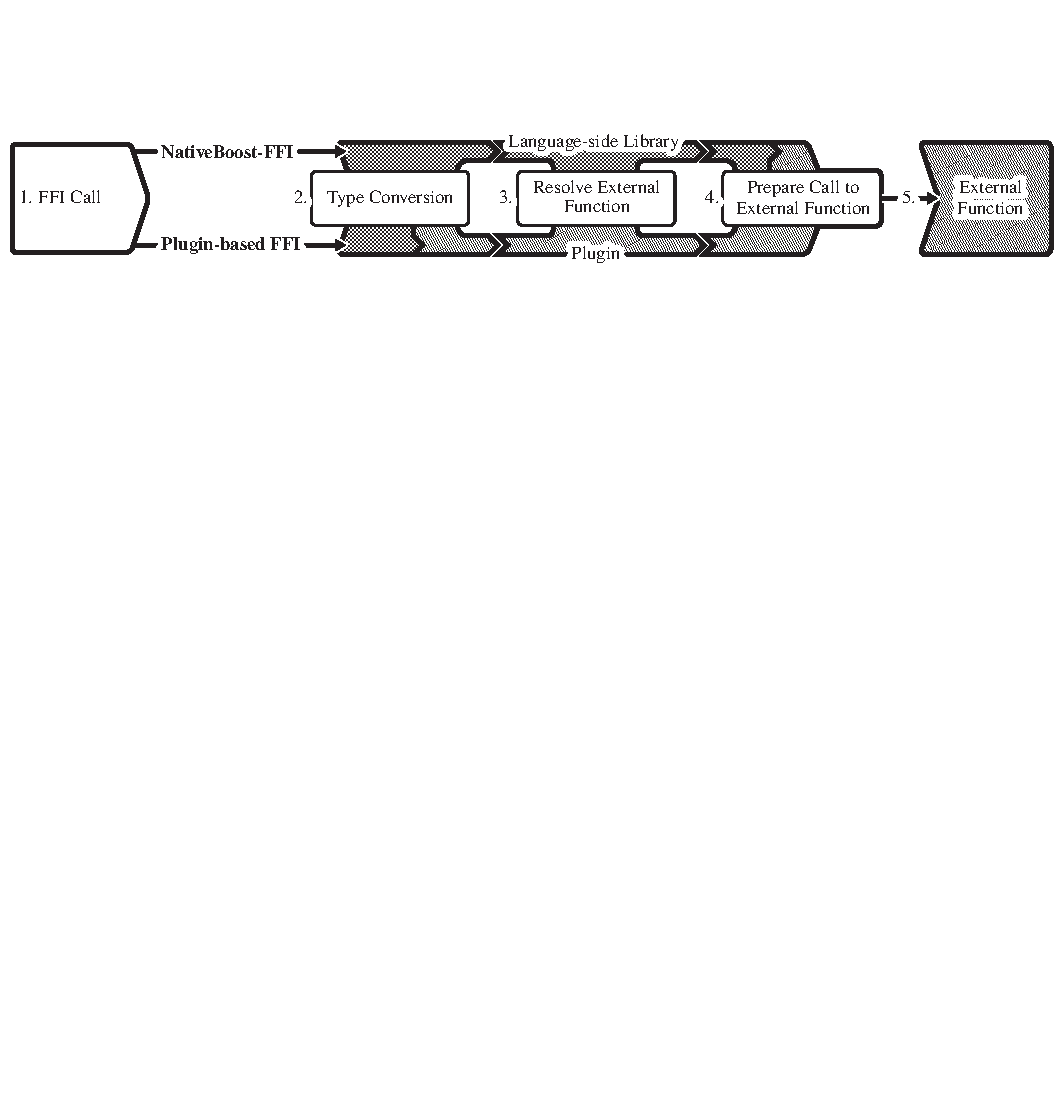
\includegraphics[width=\linewidth]{ffiOverview}
%\caption{\NB Overview: Unlike typical FFI implementations \NB only resorts to the VM-level when actually calling the external function in step 4. Typical implementations already cross the low-level barrier during the type conversions at step 2.}
%\figlabel{ffi}
%\end{figure*}

FFIs enable a programmer to call external functions without the need to implement additional VM extensions.
\NB \cite{Brun13a} is a production-ready FFI for \PH, developed on top of \B.
An FFI implementation consists of two main parts: calling external functions and converting data between the two environments.
Typically a big percentage of these two parts are implemented at VM-level with statically defined bindings.
Relying on \B's capability to dynamically generate and execute native code we developed a complete FFI at language-side.
This way the VM no longer requires to have a specific FFI extension.

%----------------------------------------------------------------------------
%\paragraph{FFI at Language-side.} 
%
%The fact that via FFI we can call external functions makes it a perfect option to replace VM extensions defined at low-level side since FFI relies only on one generic low-level extension: the language-side has to be able to generate and subsequently call native instructions. 
%A VM with a well-defined plugin infrastructure enforces the same level of separation.
%However, unlike plugins, FFI bindings are implemented without crossing a language barrier. 
%Most code for FFI bindings can be written at language-side in already existing familiar infrastructure.
%
%\revc{One sentence says "without crossing' but then the next sentence says: "Most code".}
%Furthermore, compared to a low-level plugin, a language-side library is easier to evolve and maintain. 
%\revc{Yes, writing FFI in a higher-level language has merits. A sure way of inspecing (perhaps in the Smalltalk debugger) the constructed stack frame would be great.}
%
%FFI-based language extensions also provide a certain level of portability.
%Often the only artifact that has to be ported is the FFI plugin for the VM.
%In the optimal case the high-level FFI code is completely compatible.
%If the platform does not provide the same signature for the function, only the language-side code requires changes.
%This is preferable since the language-side part of the FFI code relies on better abstractions and infrastructure for debugging.
%\NB does not even depend on a specific VM plugin but on the generic infrastructure provided by \B.
%All the FFI is implemented at high-level language-side. 
%\del{Figure \figref{ffi} shows how only the last step in calling an external function relies on low-level VM interaction.}
%Section \secref{ffi-low-level} explains the execution component details.
%Via reflection techniques \NB provides a simple yet powerful marshalling library which is further described in Section \secref{ffi-symbiosis}.
%
%----------------------------------------------------------------------------
%\subsubsection{\NB in a Nutshell.}
%\seclabel{ffi-nutshell}
%----------------------------------------------------------------------------
A very simple example to illustrate the functionality of \NB is to access the current environment variables with the \ttt{getenv} C function.
\ttt{getenv} takes a name as single argument and returns the value of that environment variable as a string:
%
\begin{stcode}{4}
getenv: name
    ^ FFI call: 'String getenv(String name)'
\end{stcode}
%
In this example \NB automatically detects, using reflection, that the argument for the \PH method corresponds to the one of the low-level C function.
The most important aspect about this example is that it is written with standard \ST code, a property that extends to almost the complete implementation.
\NB, additionally to the native code activation, relies on two simple primitives provided by \B to retrieve addresses of external functions (\ttt{dlsym}) and to load external libraries (\ttt{dlopen}).

\NB generates the glue code to call external functions dynamically at run time.
It relies on \B's features presented in Section~\secref{benzo-language-side} to generate and activate native code at runtime.
This gives \NB a significant advantage over static approaches: the generated native code is specific to the callout.
For instance in the \ttt{getenv} example, the marshalling code for converting from the internal \PH strings to C strings is written a small assembler routine.
In this specific context, the assembler code is faster than any language-side code.
Yet \NB is very flexible since all these conversion routines are defined at language-side. 
Each language-side library can define its own highly efficient conversion routines for types that are used in FFI callouts, which is not directly possible to do with a VM extension.

\cb{fill the page...}

%----------------------------------------------------------------------------
\subsection{Reflective Primitives}
\seclabel{waterfall}
%----------------------------------------------------------------------------
The Pharo VM (Cog) is developed in a language that is a subset of \ST, known as Slang, which is transformed to C and then compiled using a standard C compiler.  
Slang basically has the same syntax as \ST but is semantically constrained to expressions that can be resolved statically at compilation or code generation time and are compatible with C.
Hence Slang's semantics are closer to C than to \ST. 

The primitives of the VM are written in Slang and that is why even in a highly reflective languages such as \ST, where almost every aspect of the language is available for inspection and modification \cite{Denk10a}, primitives can not be changed at runtime. They can only be intercepted with reflective techniques with considerable performance overheads.
This is an important limitation since primitives are, in general, performance demanding components.
Waterfall~\cite{Char13a,Waterfall} is a tool that allows developers to change the code written in Slang for primitives and translate it to native code at runtime.
This replaces the indirection via C that is used in the default compilation process.
Given that Slang source code can be modified at runtime as any other \ST method, Waterfall fosters primitives to be dynamically adapted without imposing the common pure reflective techniques performance degradation.

\vspace{-3mm}
\subsubsection{Waterfall Summary.}
From a high-level point of view Waterfall provides two services which work transparently: 
%
\begin{enumerate}
	\item Compilation of Slang code on demand (lazily).
	\item A clear interface for executing, at runtime and from language-side, the native code generated.
\end{enumerate}
%
The first item allows to change the code of primitives at language-side and generate the corresponding native code when needed. %It also provides the possibility to write methods or functionalities with the same Smalltalk syntax but with a static semantic. 
%It consists essentially of a transformation toolchain that uses the AST that is generated by the standard \PH compiler harnessing that Slang and \ST have the same syntax. 
%Then this AST representation is translated to native code enforcing C-like Slang semantics. The current prototype has only three fully implemented stages: Slang to AST, AST to an IR (between TAC and SSA) and finally AST or IR to native. The design is open for future additions at any level. One typical enhancement missing is having different levels of intermediate representations with various techniques on code optimization and register allocation strategies as modern compilers propose \cite[Ch.\ 1]{Appe98a}. 
The second item enables the execution of the dynamically generated native code.
This includes for instance the finding of addresses of VM internal symbols and all the effort to link the two worlds, \ST and native.
Waterfall relies on \B for most of this low-level functionalities.
In particular \NB, the \B-based FFI presented in Section~\secref{ffi}, is used for interfacing with C libraries (\ttt{dlsym}). 

\paragraph{Primitives in Smalltalk.}
As already partially explained, whenever a method is compiled with the \ttt{primitive} pragma as shown in Section \secref{vm-interaction} a flag is set on the \ttt{CompiledMethod}. 
If the VM tries to activate such a method, instead of interpreting the bytecodes it calls the corresponding function at VM-level~\cite{Gold83a}.
%The binding between primitives and numbers is described in a table indexed by number.
Smalltalk distinguishes two types of primitives: essential and non-essential primitives.
Essential primitives are required for the bootstrapping and the essential operations of the language, such as creating a new object or activating a block.
The second category of primitives are mainly used for optimization purposes.

\paragraph{Dynamically Interchangeable Primitives.}
Waterfall uses \B's mechanism for replacing primitive methods with customized versions that are nativized dynamically as described in Section~\secref{benzo}.
The loophole described there is exploited by Waterfall to enable dynamic modification of VM behavior and hence bring primitives to life at language-side.


%----------------------------------------------------------------------------
\subsubsection{Benefits} 
We identified two main benefits of changing VM primitives at runtime:

%\begin{itemize}[noitemsep]
\begin{enumerate}
	\item Reducing VM complexity by implementing non-essential primitives reflectively at language-side.
	\item Dynamic instrumentation of primitives.
\end{enumerate}

\paragraph{Reducing VM Complexity.}
VM extensions are only justified in the presence of strong performance requirements (see Section~\secref{related}).
All non-essential primitives fall into this category.
Using Waterfall, these primitives can be implemented at language-side.
This means that these primitives become first-class citizens of the high-level environment and thus evolve with less effort.

\paragraph{Essential Primitives.}
For essential primitives the previous argument does not hold since a static version is needed for a correct startup of the system.
%These primitives can not be fully replace by a language-side implementation using Waterfall.
%For instance, essential primitives are required for system startup.
They would trigger an endless recursion when booting up the system and trying to generate them using Waterfall at the same time.
However, nothing prevents from replacing essential primitives at runtime with customized versions, once the system startup is completed. 

\paragraph{Why do we need better instrumentation?}
Instrumentation of essential primitives from language side is an error-prone task falling in many cases in non-termination due to recursive loops. 
An example of this behavior, can be observed when changing the essential \ttt{basicNew} primitive, which is responsible for instantiating new objects.
Even a very simple instrumentation task such as printing the address in memory of the created object is problematic.
If during the printing process another object is created the very same instrumented \ttt{basicNew} primitive would be triggered.
Using reflective techniques it is possible to avoid this loop, however, with a considerable overhead.
With Waterfall we can forget about these issues since the instrumentation code will be implemented at the lowest level.
On section \secref{wf-performance} we show how Waterfall, the \B based approach for generating primitives on the fly, outperforms the reflective solutions for primitives instrumentation. 

%
%\revb{Here, you should also have explained for what purposes those primitives are instrumented. Giving a few examples that cannot be achieved without primitive instrumentation would be sufficient. 5.2.3 performance of instrumentation should also be justified through the performance of an instrumented program that is used in practice.}
%\gc{I have been working in a wf paper more oriented to efficient code. for eg, dynamic and on demand plugins. So i'm more focused %to other direction now. Resuming this examples will not be easy. If you think it is %completely neccesary i can try benchmarking this but only one reviewer from 5 is asking for it.}
%
%Actually it is absolutely possible to do instrumentation completely at language-side for non-essential primitives without Waterfall by accepting the performance penalty, but for essential primitives doing it is a very fragile task.
%The chances of accidentally invoking the same primitive in the language-side instrumentation code are high.
%Without very careful design the instrumentation code will thus trigger an endless recursion. Also performance issues could be prohibitive for language-side solutions.

%----------------------------------------------------------------------------
\subsubsection{Waterfall Future.}
\cb{filling the page with the future outlook, maybe mention that it might make sense to extend waterfall further down}
Currently Waterfall reimplements all Slang arithmetic essential operations statically as native code templates.
The existing JIT of the Pharo VM does exactly the same for performance reasons.
This is code duplication and should be avoided.
With the language-side JIT compiler described on next section we can reuse the same code. Another plan for Waterfall is to use it for disconnecting most plugins defined at Slang side from the VM compilation process and dynamically nativize them on a lazy approach.
Finally, adding stages to the compiler with different levels of intermediate representations and applying optimizations to each would bring its performance closer to completely low-level optimized primitives.

%\revc{It appears that Waterfall can only replace the definitions of functions that have entries in the primitive table. But one could imagine that it could be useful if the programmer can customize somewhat deeper level of implementation, such as the logic of method look up (to plug in a different method cache logic for example). Allowing this could be another future work.}

%\cb{refer to the customized lookup paper for smalltalk/X with cache structures being passed to the user and the next section actually, since we customize the COMPLETE instruction generation with high-level code}


%----------------------------------------------------------------------------
\subsection{Nabujito JIT Compiler}
\seclabel{nabujito}
%----------------------------------------------------------------------------
\cb{try to strip away some text to make it fit on 2 pages}
In this section we present Nabujito, a \B-based approach for a language-side JIT compiler.
Nabujito goes even further than Waterfall using almost the same techniques.
However, instead of focusing on primitives, Nabujito generates native executable code for standard \ST methods.
Primitives tend to be more low-level, whereas Nabujito focuses on high-level \ST code. 


%----------------------------------------------------------------------------
\subsubsection{The JIT of the Pharo VM.}
The \PH VM (Cog) already comes with a JIT that translates bytecodes to native instructions.
It transforms \ST methods into slightly optimized native code at runtime.
The main speed improvement comes from avoiding bytecode dispatching and by inlining certain known operations and primitives \cite{Ayco03a}.
The most complex logic of the JIT infrastructure deals with the dynamic nature of the \ST environment.
Methods and classes can be changed at runtime and that has to be addressed by the JIT infrastructure.
The JIT compiler, by which we refer in this context to the transformation of bytecodes to native code, represents a small part of the whole infrastructure.
There exists more important stages as an additional register allocation pass to reduce the number of stack operations \cite{Mira99a,Mira11a}.
The existing JIT infrastructure is implemented in Slang \cite[Ch.\ 5]{Blac09a} as the rest of the VM.

%----------------------------------------------------------------------------
\subsubsection{Limitations of VM-level JIT Compilers.}
In the context of Nabujito we separate a JIT infrastructure into separate parts.
The major part is to have a VM that uses stack-mapping.
In the case of a bytecode-based interpreter, we assume that the VM provides routines to switch between a bytecode interpretation context and a low-level native execution context.
With Nabujito we move the JIT compiler,the part that generates native code at runtime, from the VM to the image.%, the part that generates native code at runtime, typically from bytecodes.
 Since the JIT compiler is quite decoupled from the rest of the JIT infrastructure we believe that a hard-coded static and low-level implementation is not optimal for several reasons:

%\begin{itemize}[noitemsep]
\begin{itemize}
	\item Optimizing \ST code requires strong interactions with the dynamic environment.
	\item Accessing language-side properties from the VM-side is hard.
	\item Changing the JIT compiler requires changes at VM-level.
	\item The JIT reimplements primitives for optimization reasons resulting in code duplication.
\end{itemize}

\paragraph{Optimization Limitations for \PH.}
In \ST methods tend to be very small and it is considered good practice to delegate behavior to other objects.
This implies that several common optimization techniques for static languages do not work well.
Dynamic method activation does not provide enough context for a static compiler to optimize methods.
Hence after inline caches and register allocation the next optimization technique is inlining.
However, inlining in a dynamic context is difficult and requires hooks at VM-level to invalidate native code when the language-side changes.
Since in \PH, compiling a method to bytecode is handled completely with language-side code most of the infrastructure to get notified about method changes is already present.

\paragraph{Primitives in the Existing JIT.}
The existing JIT reimplements the most used primitives at VM-level.
This guarantees that the VM stays as long as possible in the JIT context (see Section~\secref{jit-interaction}). Additionally this enables new performance optimizations that for instance are hard to achieve with standard compliant C code.
A typical example is the integer addition which has to deal with overflow checks and conversion of tagged integers.
In Section \secref{waterfall} we describe how Waterfall suffers a similar constraint. Waterfall manually defines such primitives in terms of native assembler instructions through the language-side \B interface.
Nabujito reuses the same optimized primitives so we rely on a single optimized definition which is shared amongst all native code libraries.

%----------------------------------------------------------------------------
\subsubsection{Implementing Nabujito.}
Nabujito is an experimental JIT implementation which replaces the bytecode to native code translation of the existing JIT infrastructure with a dynamic language-side implementation.
Nabujito is implemented mainly with a visitor strategy over the existing intermediate bytecode representation. 
Additionally we reimplemented vital native routines for the JIT which are not directly exported by the VM using \B. 
Nabujito relies on the following VM-level infrastructure to manage and run native code for any \PH method:

%\begin{itemize}[noitemsep]
\begin{itemize}
	\item Fixed native code memory segments.
	\item Routines for switching contexts.
	\item Native stack management.
\end{itemize}

\paragraph{Dynamic Code Generation.}
%To simplify the implementation we decide to manually trigger JIT compilation.
%For primitives known by Waterfall we rely on that infrastructure to generate the native code.
For standard methods Nabujito takes the bytecodes and transforms them to native code.
It also applies optimizations such as creating low-level branches for \ST level branching operations like \ttt{ifTrue:}.
Optimizations for additional methods are all implemented flexibly at language-side.
Wherever possible, we reimplement the same behavior as the existing native JIT compiler.
Eventually the native code is ready and \B attaches it to the existing compiled method.
When the language-side jitted code is activated \B ensures that we do not have to leave the JIT execution mode, and thus we can call methods at the same speed as the existing JIT.
%The benchmarks of section \secref{nabujito-performance} show the empirical results.

%----------------------------------------------------------------------------
\subsubsection{Outlook.}
One major performance optimization missing in both, the original \PH VM-level JIT and Nabujito, is inlining. 
By inlining we are able to create methods that are potentially big enough for optimizations.
However, inlining is a difficult task in a highly dynamic language such as \ST or Self \cite{Cham89a}. 
Efficient inlining can only be performed with sufficient knowledge of the system. 
Accessing this high-level information from within the VM is cumbersome and requires duplication of language-side reflective features.
The JIT lives on the same level as the information it needs relying on the already present reflective features of Smalltalk.


%----------------------------------------------------------------------------
\section{Performance}
\seclabel{issues-performance}
%----------------------------------------------------------------------------
\B allows the generation of speficic and thus efficient native code.
In Section~\secref{benzo} we explained how \B causes only a one-time overhead for native code generation. 
Thereafter it is cached for later activations.
The three usecase presented in Section~\secref{usecase} heavily benefit from this fact.
Even though the code generation at language-side is generally slower than a C-level implementation, the overhead can mostly be neglected.
Even better, for instance the \B-based FFI implementation presented in Section~\secref{ffi} outperforms a VM-level FFI-plugin due to a more flexible language-side implementation. 
These results are shown in the following Table \tabref{ffi-performance-simple}.

The rest of this section discusses in more details the performance of our three \B-base usecases: an FFI, dynamic primitives and a language-side JIT compiler.
%Unless stated otherwise, the performance evaluation is based on using SMark\, a benchmarking framework which measures 

% ---------------------------------------------------------------------------
\subsection{\B-based FFI}
% ---------------------------------------------------------------------------
\seclabel{nb-performance}

Compared to a static plugin-based FFI implementation \NB has only a one-time startup overhead with its numbers shown in Section~\secref{issues-performance}.
Generating the native code at language-side is substantially slower than directly setting up all the conversions and calling the external functions from C code. 
In some cases the penalty for some compilation effort on \NB is as high as a factor of 100 compared to classic approaches.
Under the assumption that the method is called several times this overhead may be considered negligible.
An in-depth evaluation of NativeBoost comparing against other solutions, is presented in a separate paper~\cite{Brun13a}.
The following table contains a performance comparison of three different FFI implementations for \PH that represents the typical showcase.

\vspace{-3mm}
\begin{table}[!ht]
    \centering
    \begin{tabular}{rlr}
                    & Call Time                        & Relative Time \\\midrule
        \NB         & \ttt{10.53} $\pm$ \ttt{0.35} ms  &  $1.0\times$ \\
        Alien       & \ttt{31.09} $\pm$ \ttt{0.94} ms  & $\approx 3.0\times$ \\
        FFI         & \ttt{19.55} $\pm$ \ttt{0.64} ms  & $\approx 1.9\times$
    \end{tabular}
    \caption{Different FFI implementations in \PH evaluating 
    \ttt{abs(int)}. Alien does marshalling at language-side while FFI does everything in C.}
    \tablabel{ffi-performance-simple}
\end{table}
\vspace{-5mm}

Table \tabref{ffi-performance-simple} measures the accumulative time of 100'000 FFI calls.
Included in these numbers is at least one additional \ST message send to activate the \NB method containing the actual call to the C function.
Each benchmark itself is run 1000 times and the average and standard deviation is taken.
We also measured calls with more complex type conversions where the performance boost against Alien pronounced even more because \NB's language-side marshalling is nativized.
The JIT interaction described in Section \secref{jit-interaction} is also an important optimization factor especially when calling out small helper routines where the context switch from jitted mode is not negligible.



% ---------------------------------------------------------------------------
\subsection{\B-based Dynamic Primitives}
% ---------------------------------------------------------------------------
\seclabel{wf-performance}

For comparing performance we implement a very simple integer operation primitive (\ttt{$>$}) using three different approaches.
The first approach is the implementation with Waterfall.
The second is to run the language-side implementation that is triggered whenever the standard primitive failed.
Finally the fast standard primitive provided by the VM.
We run the three approaches by measuring the cumulative time over one million primitive activations averaged over 100 runs.
The absolute numbers are less important than the relative factor between them.
We present the results of this experiment in Table~\tabref{waterfall-performance}.
%
\vspace{-3mm}
\begin{table}[!ht]
    \centering
    \begin{tabular}{rrr}
					& Running Time 						& Relative Time \\\midrule
		VM			& \ttt{  6.4}  $\pm$ \ttt{0.14} ms & $1.0\times$\\
		Waterfall	& \ttt{ 22.8}  $\pm$ \ttt{0.17} ms & $\approx3.6\times$\\
        Reflective	& \ttt{195.0}  $\pm$ \ttt{0.16} ms & $\approx30.0\times$
    \end{tabular}
    \caption{Comparing running time of different implementations of integer arithmetic primitive.}
    \tablabel{waterfall-performance}
\end{table}
\vspace{-5mm}
%
As expected Waterfall's solution outperforms pure reflective one by factor $9$ to $10$.
Waterfall clearly outperforms a purely reflective solution since all the meta programming overhead for the intercession mechanism is avoided. This results thus makes a whole new set of runtime extensions feasible that were previously limited by their strong performance penalty.
Furthermore the performance penalty over a completely optimized VM solution that has extreme optimization techniques, such as inlining and register allocation, is less than a factor of $4$.
Applying standard optimization techniques, not yet implemented in Waterfall, will almost sure improve these numbers even more.
A more detailed analysis of Waterfall is available separately \cite{Char13a}.

% ---------------------------------------------------------------------------
\subsection{\B-based JIT compiler}
% ---------------------------------------------------------------------------
\seclabel{nabujito-performance}

The performance evaluation for our \B-based JIT compiler is focused on the language-side code-generation part.
Nabujito essentially generates the same native code as the VM-level JIT, hence there is no performance difference at evaluation time.
However, Nabujito is clearly slower during the warm-up phase.
Compilation of the native instructions will take considerably more time compared to the VM-level implementation of the same bytecode to assembler transformation.
The cost of transforming the bytecodes to native code at VM-level can be measured in native instructions, whereas the unit at language-side is bytecodes.
However, we point out again, that this is a one-time overhead.
From the in-production experience of NativeBoost, the \B-based FFI (see Section~\secref{nb-performance}), we know that these costs amortized, especially for long-term applications.
Instead of focusing on the final performance of the generated code, we present the compilation time compared to the normal \PH bytecode compiler, which also resides at language-side.

\begin{table}[!ht]
    \centering
    \begin{tabular}{rll}
                      & Compilation Time \\\midrule
        \PH Compiler  & \ttt{71} $\pm$ \ttt{1} ms   \\
        Nabujito      & \ttt{73} $\pm$ \ttt{1} ms
    \end{tabular}
    \caption{Compilation efforts of the standard \ST compiler in \PH and Nabujito for the a simple method returning the constant \ttt{nil}.}
    \tablabel{nabujito-performance-small}
\end{table}
\vspace{-5mm}

In Table \tabref{nabujito-performance-small} we compare the compilation speed of the standard \PH compiler and Nabujito.
We measure the accumulated time spent to compile the method 1000 times.
The average and deviation are taken over 100 runs. 
The \PH compiler takes source code as input and outputs \ST bytecodes.
Nabujito takes bytecodes as input and outputs native code.

We see that in the simple case displayed in Table \tabref{nabujito-performance-small} Nabujito's compilation speed lies within the same range as the standard \ST compiler.
We expect that in the future we apply more low-level optimizations and thus increase the compilation time of Nabujito.
However, we have shown in the performance evaluation for \NB, the \B-based FFI, in Section \secref{nb-performance} that even a rather high one-time overhead is quickly amortized.
Furthermore with Smalltalk's image approach the generated native code is persistent over several sessions.
A subsequent restart of the same runtime will not cause the JIT to nativize the same methods it did during the last launch.
Hence our approach is even valid for short-timed script-like applications as most of the methods will already be available in optimized native code from a previous run.


% ===========================================================================
\section{Related Work}
\seclabel{related}
% ===========================================================================

In the context of \B we have to respect a variety of related work spawning different abstraction levels.
On a more abstract scale \B allows for a new way of extending the complete language runtime, hence we classify the related work according the following categories show in Figure~\figref{extensionComparison}: general language-side extensions, extensions using reflection, VM-level extensions, and hybrid approaches.
%
%We present now an overview of the approaches used to extend a language runtime and expose their limits.
%High-level languages are in general sustained by a VM and a vast set of libraries written in the language itself. 
%Extending or improving the existing language runtimes is a difficult task.
%In most cases the VM is considered as a black box.
%Additionally the VM is written in a completely different language using another abstraction level than the one it supports.
%Typically high-level language VMs are written in C or C++.
%To address extensions in this context there exist some known approaches:
%
%\begin{description}[noitemsep]
%	\item[Language-side Library] based on implementing a new or existing library. 
%	\item[Language-side Reflective Extension] relying on reflective features of the language. 
%	\item[VM Extension] by writing plugins or changing the core of the VM.
%	\item[Hybrid Extension] by accessing external libraries using FFI.  
%\end{description}
%

%The relation between the side concerning the abstraction and implementation levels (VM vs. Language) of these extensions is illustrated in Figure \figref{extensionComparison}.

\begin{figure}
	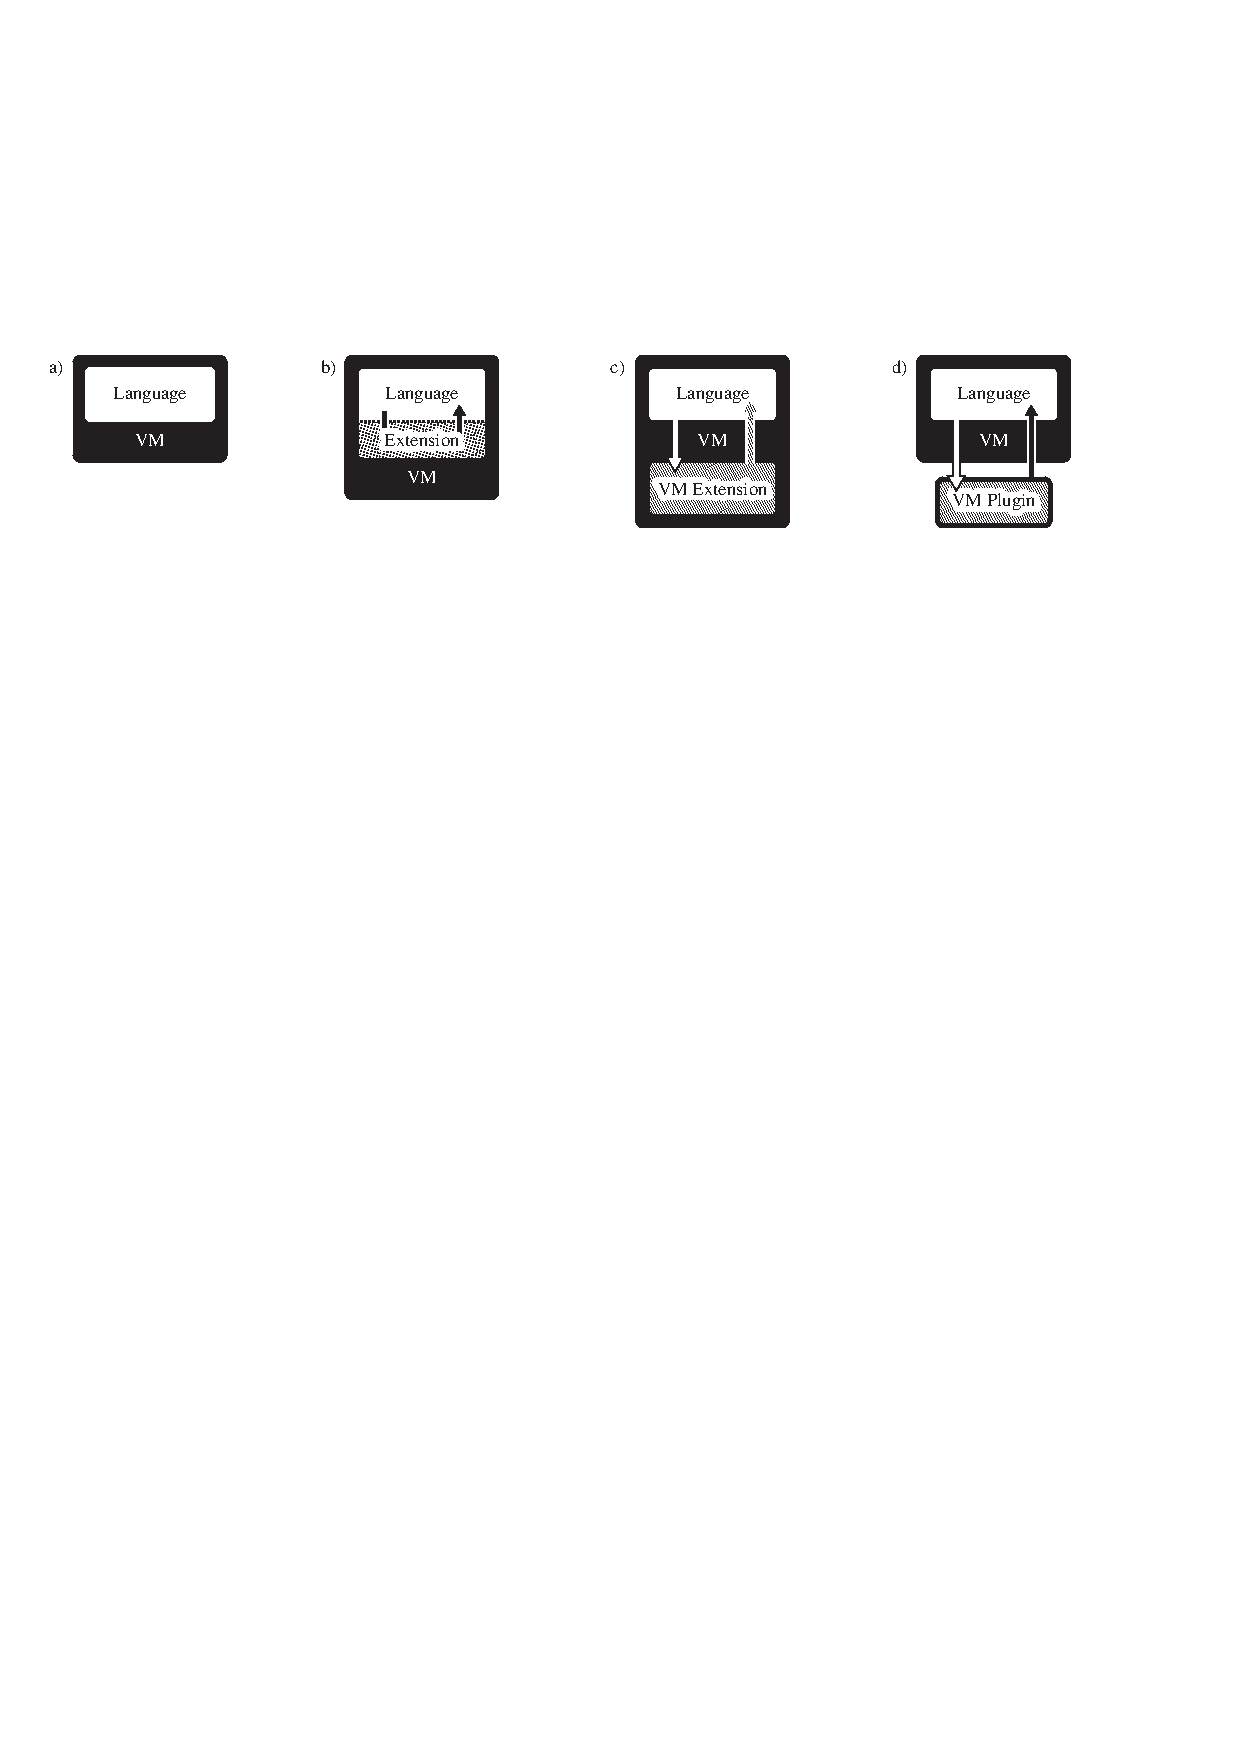
\includegraphics[width=\linewidth]{extensionComparison}
	\caption{Comparing different extension mechanisms: 
		a) language running on a standard VM, 
		b) language-side implementation of an extension
		c) language using features from a VM extension, 
		d) language using features from a separate VM plugin.}
	\figlabel{extensionComparison}
\end{figure}
\vspace{-5mm}

%----------------------------------------------------------------------------
\subsubsection{Language-side Library.}

The most straight forward solution for extending a language is to write libraries within the language itself. 
This option provides the advantage that the aggregate behavior is accessible and evolvable for any language developer.
However, language-side libraries are constrained by the underlying managed language runtime.
The VM separates the language from the low-level internal details.
As a consequence language-side libraries are not feasible for all feature requirements.
For instance the previously mentioned example of instrumenting the language runtime is not possible as a standard language-side extension without a considerable performance loss.
So, even though we prefer extensions and optimizations at language-side, there are certain limitations of a managed language runtime that can not be circumvented.
If all language-side optimization opportunities have been exhausted it is exposing the need to resort to lower level approaches.
%\\

%\noindent\emph{Language-side libraries are constrained to the capabilities of the underlying VM and thus not general enough. Additionally not all performance bottlenecks can be addressed at language-side.}

%----------------------------------------------------------------------------
\vspace{-2mm}
\subsubsection{Language-side Reflective Extensions.}

This is a subcase of the previous approach but in the context of reflective environments that expose particular characteristics.
For instance, Meta Object Protocols (MOP) \cite{Kicz91a} based on reflection \cite{Maes87a} are used to define certain control points in the system to change the language.
By composing meta objects it is possible to even modify the semantics of the language. 
Several languages such as Smalltalk, Python, and others provide reflective capabilities with different depths \cite{Ande98a,Flan08a,Van10a}.
However, most modern programming languages only have very limited support for intercession.
Hence the possibilities for dynamically changing language semantics or features are limited. 
Furthermore reflective capabilities are hard to implement efficiently.
Reflection imposes substantial performance penalties on most computations by postponing bindings \cite{Male96a}. 
Nevertheless, there are exceptions for a subset of reflective behavior which are implemented efficiently using a high-level MOP \cite{Vran12a}.
Though these approaches remain as a few exceptions.
In the typical low-level VM it is difficult to gain reflective access to language-side objects.
Similar to the previous case, our goal is to extend language features in a general way and it was shown that this is only partially possible by reflective extensions. 
%\\

%\noindent\emph{Reflective capabilities are not enough for general extensions. Even when suitable, they usually pose a significant performance overhead up to the point where they become unfeasible.}

%----------------------------------------------------------------------------
\vspace{-2mm}
\subsubsection{VM Extensions.}
\seclabel{vm-extensions}

Another approach is to attach plugins to the VM.
Plugins are direct bindings to external libraries described at VM-side or libraries linked to the VM executable \cite[Ch.\ 5]{Blac09a}. 
They provide a performance boost in comparison to pure language-side solutions.
Using highly optimized native libraries it is straightforward to outperform code written at language-side.
However, plugins are commonly written in the same language as the VM, at a low abstraction level.
Few exceptions are self-hosted languages \cite{Unga05a,Wimm13a,Rigo06a}.
To support a fluent development process, VMs should come with an infrastructure for building extensions at same abstraction level than the language.
Instead they tend to be very complex and to have sluggish building processes. For example, only a few VMs have high-level debugging facilities \cite{Inga97a,Unga05a,Wimm13a}.
Also from a VM maintenance point of view, extensions have to be avoided if possible and should only be used for critical performance issues that can not be properly addressed at language-side.
An example of how the complexity of the VM can affect development efforts is the core of the Self VM \cite{Unga07a}.
After reduced development resources parts of the complex but efficient compiler infrastructure had to be abandoned in favor of a more maintainable code-base.

\todo{properly integrate}
High-level low-level programming \cite{Fram09a} encourage to use high-level languages for system programming.
Frampton et al. present a low-level framework packaged as \textsc{org.vmmagic}, which is used as system interface for Jikes, an experimental Java VM.
Additionally their framework is successfully used in MMTK \cite{Blac04a} which is used independently in several other projects.
The \textsc{org.vmmagic} package is much more elaborate than \B but it is tailored towards Java with static types.
Methods have to be annotated to use low-level functionality.
Additionally the strong separation between low-level code and language-side application does not allow for reflective extensions of the language runtime.
Finally, they do not support the execution nor generation of custom assembly code in the fly.

Other related approaches are VM generation frameworks in general.
They try to abstract away the complexity of the VM and use high-level languages as compiler infrastructure.
A very successful research project is Jikes Research VM \cite{Jikes}.
It uses Java to metacircularly define a Java environment which then generates the final VM.
A similar framework is PyPy \cite{Rigo06a} a VM framework including an efficient JIT. 
PyPy uses a restricted subset of the Python language named RPython which is then translated to various low-level backends such as C or LLVM code.
There exist several different high-level language VM implementations on top of PyPy such as \ST \cite{Bolz08a} or Prolog.
However, its main focus lies on an efficient JIT generator mainly for a Python interpreter, and not on a direct, language-side assembler interface.


%----------------------------------------------------------------------------
\vspace{-5mm}
\subsubsection{Hybrid Extensions.}
The last approach is to reuse an existing library usually implemented in a foreign language.
The languages interact through a well-defined Foreign Function Interface (FFI).
FFI-based extensions are an hybrid approach between pure language-side extensions and VM-side ones.
Interaction with native libraries is supported by a dedicated VM functionality for calling external functions.
This allows for a smooth interaction of external code and language-side code.
FFI based extensions share the benefits of a maintainable and efficient language-side library with modest implementation efforts.
However, FFI is only a bridge or interface for allowing the interaction of different languages. 
It is not possible to directly synthesize new native features from language-side.
For this purpose we have to interact with a custom-made native library.
From an extension point of view this is close to the VM extensions discussed previously.

Additionally to the interface limitations, there exists a performance overhead in FFI for making the interaction between different languages possible. 
This is due to marshalling arguments and types between both languages \cite{Fish00a,Repp06b}.


Other high-level languages such as Lua leverage FFI performance by using a close interaction with the JIT.
LuaJIT \cite{luaffi} for instance is an efficient Lua implementation that inlines FFI calls directly into the JIT compiled code.
Similar to \B this allows to minimize the constant overhead by generating custom-made native code.
LuaJIT is mainly written in C which has clearly different semantics than Lua itself.
Compared to \ugh{our} approach the efficient VM implementation suffers from the shortcomings described in Section \secref{vm-extensions}. 

Kell and Irwin \cite{Kell11a} take a different look at interacting with external libraries.
They advocate a Python VM that allows for dynamically shared objects with external libraries.
It uses the low-level DWARF debugging information present in the external libraries to gather enough metadata to automatically generate FFIs.
However, they do not focus on the reflective interaction with low-level code and the resulting benefits. 

QUICKTALK \cite{Ball86a} follows a similar approach as Waterfall.
However, Ballard et al. focus mostly on the development of a complex compiler for a new \ST dialect.
Using type annotations QUICKTALK allows for statically typing methods.
By inlining methods and eliminating the bytecode dispatch overhead by generating native code QUICKTALK outperforms interpreted bytecode methods.
Compared to Waterfall QUICKTALK does not allow to leave the language-side environment and interact closely with the VM.
Hence it is not possible to use QUICKTALK to modify essential primitives.

A notable exception to the metacircular VMs mentioned earlier is the Self implementation Klein \cite{Unga05a}.
Unlike typical other metacircular approaches it does not strictly separate compile-time and runtime.
The reified VM concepts are available at runtime, which is a result from implementing the typical VM pieces at language-side.
Compared to our approach, Klein's bridging efforts are much more complete.
However, Klein is built on a completely new VM infrastructure, whereas \B requires only few changes to achieve its functionality.


% ===========================================================================
\section{Conclusions}
\seclabel{conclusion}
% ===========================================================================

We presented \B, an integral approach for reflective high-level low-level programming.
Using \B we efficiently implemented at language-side three distinct language feature extensions that typically reside at VM-level.
\B promotes a smooth and powerful interaction with the low-level world by dynamically generating native code from language-side.
This enables to exploit the underlying platform capabilities only when strongly needed without leaving the development platform and through a high-level programming interface. 
As a result, \B advocates the use of development tools and abstraction level of the high-level language for as much as possible or desired.

By combining high-level reflection capabilities with efficient low-level code we manage to do dynamic primitive instrumentation and reuse the code for primitive operations which is duplicated on the standard JIT approach.
We also show that since \B caches native code transparently at language-side our JIT compiler poses only a one-time overhead when generating native code. 
Finally, we also show how our mature FFI implementation outperforms an existing C-FFI implementation by a factor of 1.5 even though we control every aspect from language-side.


As a final conclusion, \B shows that promoting clear interfaces for controlling low-level code completely from language-side produces efficient solutions for system programming requirements without resorting to pure low-level solutions.
We showed that fostering the abstraction provided by high-level languages and resorting to the system programming capabilities of low-level languages only when completely needed is not only possible but profitable.
Furthermore we manage to considerably reduce complexity and code duplication which results in better maintainability.



% =============================================================================
\ifx\wholebook\relax\else
    \end{document}
\fi